%!TEX root = ../report.tex
\section{Joystick Review} % (fold)
\label{sec:joystick_review}

Joysticks are devices which allow a user to control a point in a "virtual map" to get a certain output (be it the point moving a component in real life, or purely virtually) based on the input to the joystick (ie. its current orientation). Simple joysticks may be used for applications from gaming simulators to basic telemanipulation to RC control. In this report it is joysticks with force feedback that are being looked at.

Haptic joysticks give the user feedback based on their inputs, an example being mechanical aircraft joysticks which give the pilot feedback based on the direction of their flight path. Without this feedback, it would be comparable to driving a racing car without the feeling of the road, an incredibly dangerous experience. In commercial use however, force feedback joysticks are limited, especially at a low price point, due to their previous limited applications. The use in medicinal technology is on the rise such that now further research and development in them is required.


\subsection{Joystick Mechanisms} % (fold)
\label{sub:joystick_mechanisms}

There are many types of joystick dependent on the necessary application. Varying from a single degree of freedom which could purely control speed, to 2DOF for dual axis positional control, and upwards. The mechanisms for these varies massively for different degrees of freedom and different uses. A single axis joystick will be a simple rotation, dual axis rotation about two axes, etc. Naturally the more axes, the more complex the system and the higher some factors are, ie inertia, and noise levels.

% subsection joystick_mechanisms (end)

\subsection{Button Joystick} % (fold)
\label{sub:button_joystick}

Perhaps the simplest type, the button joystick relies on four pressure sensitive contacts which can be pressed either alone, or together to give a variety of responses. These were used in early games consoles and basic RC controllers. An example can be seen in Figure~\ref{fig:button_joystick}.

\begin{figure}
  \centering
  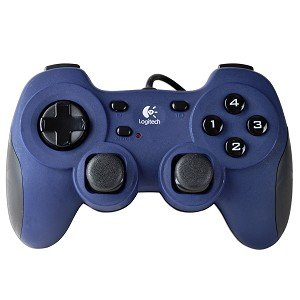
\includegraphics[width=0.5\textwidth]{button_joystick.jpg}
  \caption{Button Joystick}
  \label{fig:button_joystick}
\end{figure}

% subsection button_joystick (end)

\subsection{Continuous "track" Joystick} % (fold)
\label{sub:continuous_joystick}

The track, or gimbal joystick is the basis of almost all modern games controllers. The joystick itself pivots about a ball mechanism and extends beyond it. The extension rests in two tracks connected to potentiometers, which, when they are moved are able to give a reading of the location of the joystick in space. See Figure~\ref{fig:continuous_joystick} for further details.

\begin{figure}
  \centering
  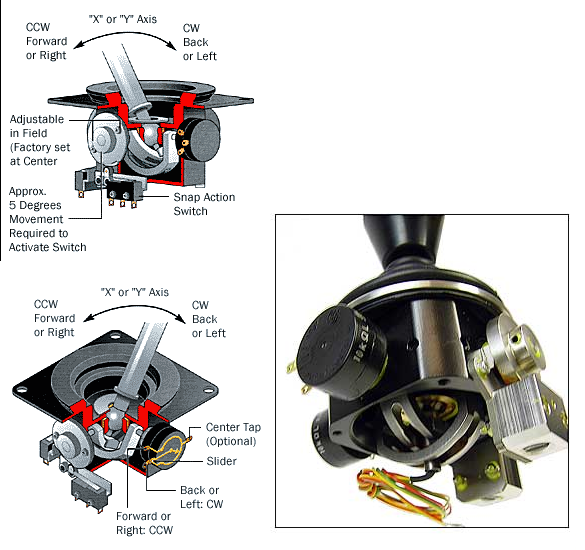
\includegraphics[width=0.5\textwidth]{continuous_joystick.png}
  \caption{Continuous Joystick}
  \label{fig:continuous_joystick}
\end{figure}

This method is compact, but has complex moving parts and can suffer from higher inertia. It is however very cheap and easy to produce. A mechanical two axis system is of most relevance to us due to its price point, and ease of use.

% subsection continuous_joystick (end)

\subsection{Accelerometer and sensor based "position tracking"} % (fold)
\label{sub:accelerometer_and_sensor_based}

A slightly newer form of controller, adopted in many forms of controllers due to its ability to be used in any position and multiple degrees of freedom. Perhaps the most mainstream use of this is in the Nintendo Wii games joystick. These use motion control and accelerometers to measure how far they have moved and in which direction in space, giving them an awful lot of freedom for movement in space. Whilst they can be accurate, expensive position sensors are normally needed, as well as a good form of calibration. These can suffer from a number of downfalls, most notably the trick of learning how to carefully use them in complex environments. Limiting the number of degrees of freedom per joystick can be seen as advantageous due to being simpler to control. They can also suffer from low accuracy and repeatability of position if there is any interference.

It is also possible to have external sensors measure movements of a person in space, ora person holding set instruments in space. These work by a light source illuminating the object, and sensors measuring the distance the light travels to each part of the object. These points are then interpreted and mapped in relevant software. Whilst relatively accurate, for very fine movements, the precision of a system like this can falter. It is also not possible to get force feedback from a design like this.


% subsection accelerometer_and_sensor_based (end)

\subsection{Trackball} % (fold)
\label{sub:trackball}

Another type of 2D joystick, however also quite difficult to control.
As depicted in Figure~\ref{fig:trackball}, trackballs protrude from the casing and are able to rotate in any direction, and move continuously allowing for fast movement.
The position is measured by small wheels on the inside of the casing that move with the ball due to friction.
It is possible to add haptic feedback to a system like this, although due to the necessary size of the positionsensing wheels, hard to get a desired feedback.

\begin{figure}
  \centering
  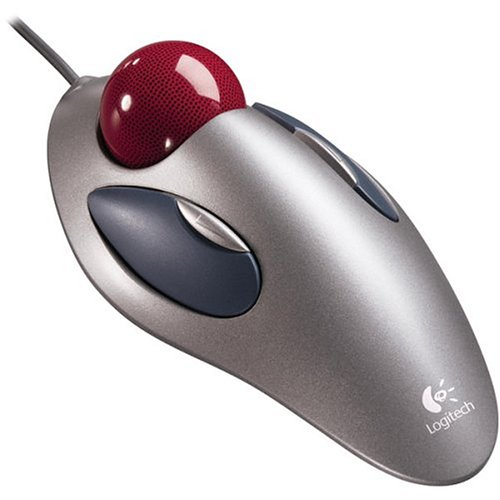
\includegraphics[width=0.5\textwidth]{trackball.jpg}
  \caption{Trackball}
  \label{fig:trackball}
\end{figure}

% subsection trackball (end)

\subsection{Summary} % (fold)
\label{sub:summary}

There are in fact many more forms of mechanisms, both complex and simple than the ones discussed, however these are viewed as the most relevant in the scope of this project due to the desire for a minimal inertia, cost friendly and very precise system. More research into an adequate design is shown in SECTION.

% subsection summary (end)

% section joystick_review (end)

\section{Haptic Technologies} % (fold)
\label{sec:haptic_technologies}

The force feedback is equally as important as the mechanism for this project, and researched had to be undertaken to see the quality of what is currently available. As can be seen, for our price point and application, the literature discovered is quite limited.

\subsection{High End - Da Vinci system, Omni Controller} % (fold)
\label{sub:high_end_da_vinci_system}

% subsection high_end_da_vinci_system (end)

\subsection{Mid Range - Haptic Cow, MR System} % (fold)
\label{sub:mid_range_haptic_cow_mr_system}


% subsection mid_range_haptic_cow_mr_system (end)

\subsection{Low End - Gaming devices, flight joysticks, Hapkit} % (fold)
\label{sub:low_end_gaming_devices_flight_joysticks_hapkit}

% Haptic Cow, Virtual reality, gaming devices,  and geomagic interfaces used for 3D designing. At the moment the mechatronics department is using a piece like this but it is very expensive and large -> therefore leading onto the requirement of something smaller with more basic functionalities.
% Then onto research papers and patented designs of joystick mechanisms.
% Input MR haematoglogical paper which we based our gimbal mechanism on.
% Input awesome paper medler found with springs. (explain reasons why this may be a little too optimistic for us to produce with budget limitations / can’t copy patented design)
% 3) Others that are similar to ours, other projects\\
%     Cool paper with the patent. Hapkit ; two papers I have bookmarked; first one we found with MR, but same mechanism\\
% 4) Professional ones;\\
%     Omni controller; Da vinci controller\\


% subsection low_end_gaming_devices_flight_joysticks_hapkit (end)

% section haptic_technologies (end)